\cotefile{138}
\scanpage{17}
le sous-corps (ou mieux, sous-anneau) de $\overline{Q}$
qu'ils engendrent, ext. finie de $Q$. On voit de
suite qu'il est indépendant du choix de
$s$, et que c'est la plus petite sous-ext\unsure{ension}
de $\overline{Q}/Q$ telle que $\widehat{\mathscr X}$ puisse se descendre \inserted{en $\widehat X_K$} : $K$
de façon que les él. de $S$ \unsure{deviennent} rat/$K$.
De plus la descente en question est unique,
à isom unique près. Les \unsure{autom\textsuperscript{ismes}|automor\textsuperscript{phismes}} de
$(\widehat{\mathscr X},S)$ (ou encore de $\mathscr X$) font un groupe
fini ($\hookrightarrow \unsure{\mathfrak S|\mathscr S}_S$), et ce groupe opère \unsure{bel-|bt.}\unsure{\& bien|déjà}
sur $\widehat X_K$.
% archive sheet number: 16

\scanpage{18}
Tour des rev. de Fermat $C_n$

Tour des revêtements abéliens de l'octaèdre
(considéré comme carte régulière 3-\unsure{pondérée|pondéree} $C_2$)

\deleted{\illegible{1}}

(revêtements abéliens de
$P^1\setminus(0,1,\infty)$, revêtements
diédraux et paradiédraux
....)
% archive sheet number: 17

\scanpage{19}
\diagram{\begin{tikzcd}[ampersand replacement=\&,column sep=large]
 X'=\mathbb P^1_{\mathbb Q}\arrow[r,dash]\arrow[d,"{\mu_{n\,\mathbb Q}}"'] \& \overline X'\arrow[d,dash]\\
 X=\mathbb P^1_{\mathbb Q}\arrow[r,dash]\arrow[d,dash] \& \overline X\quad 0,1,\infty,-j,-\bar j\arrow[d,dash]\\
 \mathbb Q\arrow[r,dash,"\Gamma"'] \& \overline{\mathbb Q}
\end{tikzcd}}
\[ f(z)=z^n \]
\diagram{\begin{tikzcd}[ampersand replacement=\&,column sep=small]
1\arrow[r] \& \mu_n(\overline{\mathbb Q})\arrow[r] \& \unsure{\mathcal E|\Sigma}_n\arrow[r] \& \Gamma\arrow[l,bend left=12]\arrow[r] \& 1
\end{tikzcd}}
\[ \mathcal E_n=\Gamma\mathbin{.}\mu_n(\overline{\mathbb Q}) \]

\[
\left\{\begin{aligned}
&S_0=\{0\},\quad S_1=\mu_n(\overline{\mathbb Q}),\quad S_\infty=\{\infty\}.\\
&E^+=\{z\mid z^n=-j\}\\
&E^-=\{z\mid z^n=-\bar j\}
\end{aligned}\right.
\qquad
\begin{aligned}
&\deleted{f(z)}\\
&E=\{z\mid z^{3n}=-1\deleted{\rbrace},z^n\ne-1\}
\end{aligned}
\]
\[
\begin{aligned}
R'&=\{z\mid z^n=\tfrac12\}\\
R''&=\{z\mid z^n=2\}\\
R&=\{z\mid z^n=-1\}
\end{aligned}
\qquad
\begin{aligned}
&R\\
&E\cup R=\{z\mid z^{3n}=-1\}
\end{aligned}
\]
\[
\begin{aligned}
\mathbb Q[E\cup R]&=\mathbb Q[\mu_{6n}(\overline{\mathbb Q})]\\
\rotatebox{90}{$\subset$}&\\
\mathbb Q[S_0\cup S_1\cup S_\infty]&
\end{aligned}
\]
\figure{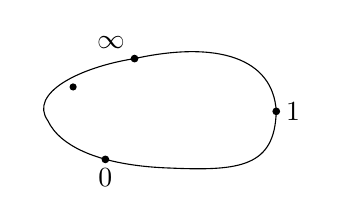
\begin{tikzpicture}[x=1cm,y=1cm]
\draw (0,0) .. controls (-.25,.35) and (.4,.68) .. (1.1,.79)
 .. controls (2.15,1.02) and (2.86,.8) .. (2.9,.12)
 .. controls (2.88,-.58) and (2.45,-.64) .. (1.55,-.60)
 .. controls (.65,-.57) and (.15,-.32) .. (0,0);
\fill (.32,.43) circle (1.3pt);
\fill (.73,-.49) circle (1.4pt) node[below] {$0$};
\fill (1.1,.79) circle (1.4pt) node[above left] {$\infty$};
\fill (2.9,.12) circle (1.4pt) node[right] {$1$};
\end{tikzpicture}}
\[
\mathbb Q[R',R'']\deleted{\unsure{R]}}=\mathbb Q[R']=\mathbb Q[\sqrt[n]{2}]
\]
\diagram{\begin{tikzcd}[ampersand replacement=\&,column sep=small]
1\arrow[r] \& \mu_{\unsure{\nu|n}}(\overline{\mathbb Q})\arrow[r] \& \Gamma'\deleted{\unsure{_n}}\arrow[r] \& (\mathbb Z/n\mathbb Z)^*\arrow[r] \& 1
\end{tikzcd}}
\[
\begin{aligned}
0,1,\infty&\mapsto0&\text{ordre }2\\
\tfrac12,2,-1&\mapsto1&\text{ordre }2\\
-j,-\bar j&\mapsto\infty&\text{ordre }3
\end{aligned}
\qquad
\begin{aligned}
\nu&=\text{ordre de }2\text{ dans }\deleted{\unsure{\mathbb Q^*}}K_n^*/K_n^{*n},\\
&\text{où }K_n=\mathbb Q(\sqrt[n]{1}).
\end{aligned}
\]
\[
g(z)=\frac{27z^2(z-1)^2}{4(z^2\unsure{-}z+1)^3}
\qquad
gf(z)=\frac{27}{4}\frac{z^{2n}(z^n-1)^2}{(z^{2n}-z^n+1)^3}
\]
\[
\lambda\frac{4}{27}=1
\]
\[
\begin{aligned}
g(z)=1&\Longleftrightarrow
\underbrace{4(z^2-z+1)^3-27z^2(z-1)^2}=0\\
&\unsure{-|=}4\big[(z+1)(z-\tfrac12)(z-2)\big]^2=4\big[(z+1)(z^2-\tfrac52+1)\big]^2\\
&\hspace{14em}=\big[(z+1)(2z^2-5+2)\big]^2
\end{aligned}
\]
% archive sheet number: 18

\scanpage{20}
\diagram{\begin{tikzcd}[ampersand replacement=\&,column sep=tiny]
D\arrow[dr,"{\text{fini}}"']\ \subset \& G_m\arrow[d,dash]\\
\&\mathbb Q
\end{tikzcd}}
\diagram{\begin{tikzcd}[ampersand replacement=\&,column sep=tiny,row sep=small]
\&\& \unsure{\bullet|0}\\
\&\& {}_n\unsure{\mathcal U|\mathcal T}\arrow[u]\arrow[d]\\
\underline{\operatorname{Hom}}(D,\arrow[d,dash] \& G_m)\arrow[d,"n"] \& {}={}\unsure{\mathcal M|\mathcal U}\arrow[d,"n"]\quad \xi\\
\underline{\operatorname{Hom}}(D, \& G_m) \& {}={}\mathcal U\arrow[d]\\
\&\& \unsure{\bullet|0}
\end{tikzcd}}

\figure{\begin{tikzpicture}[scale=.7]
\draw (0,0) .. controls (0,.6) and (.3,1.15) .. (1.08,1.58);
\end{tikzpicture}}
\[
T(\mathbb Q)\ni\xi \qquad H^1(\mathbb Q,T_\infty(\mathcal U))
\]
\figure{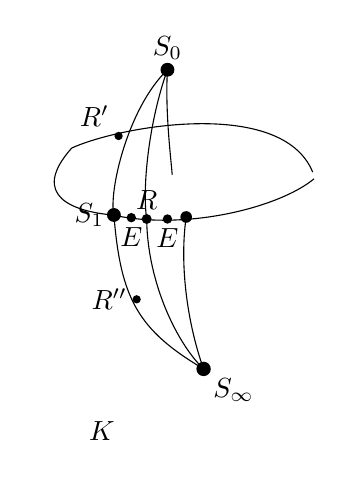
\begin{tikzpicture}[x=.85cm,y=.85cm]
\draw (3.65,.42) .. controls (3.2,1.53) and (.8,1.12) .. (.05,.78)
 .. controls (-.6,.05) and (.1,-.17) .. (.66,-.22)
 .. controls (1.75,-.46) and (3.15,-.11) .. (3.67,.32);
\draw (1.48,1.95) .. controls (.88,1.37) and (.6,.12) .. (.68,-.22)
 .. controls (.78,-1.47) and (1.04,-1.94) .. (2.02,-2.52);
\draw (1.48,1.95) .. controls (1.20,1.17) and (1.10,.18) .. (1.17,-.28)
 .. controls (1.18,-1.25) and (1.64,-2.16) .. (2.02,-2.52);
\draw (1.48,1.95) .. controls (1.44,1.28) and (1.55,.48) .. (1.55,.38);
\draw (1.76,-.25) .. controls (1.65,-1.02) and (1.8,-1.91) .. (2.02,-2.52);
\fill (1.48,1.95) circle (2.5pt) node[above] {$S_0$};
\fill (.75,.96) circle (1.5pt) node[above left] {$R'$};
\fill (.68,-.22) circle (2.5pt) node[left] {$S_1$};
\fill (.94,-.26) circle (1.7pt) node[below] {$E$};
\fill (1.17,-.28) circle (1.8pt) node[above] {$R$};
\fill (1.48,-.28) circle (1.7pt) node[below] {$E$};
\fill (1.76,-.25) circle (2.1pt);
\fill (1.02,-1.48) circle (1.5pt) node[left] {$R''$};
\fill (2.02,-2.52) circle (2.6pt) node[below right] {$S_\infty$};
\node at (.5,-3.45) {$K$};
\end{tikzpicture}}
\diagram{\begin{tikzcd}[ampersand replacement=\&,column sep=large,row sep=large]
\Gamma\arrow[r]\arrow[dr,"{\substack{\text{image de}\\\text{dim }\unsure{11|1?|n}+1?}}"'] \& \operatorname{Aff}(T_\infty(\mathcal U))\arrow[d]\\
\&\operatorname{Aut}(T_\infty(\mathcal U))
\end{tikzcd}}
Ss-groupe d'indice fini : opère \unsure{par|dans} \unsure{homothéties|hom.}

$\unsure{\xi|j}_i$ \unsure{---} \unsure{linéair\textsuperscript{t}} indép. mod \unsure{racines|premier} de 1

\diagram{\begin{tikzcd}[ampersand replacement=\&,column sep=large]
\Gamma\arrow[r]\arrow[dr]\arrow[ddr,bend right=42] \& \operatorname{Aff}(n,\widehat{\mathbb Z})\arrow[d]\quad\deleted{\text{image de}}\\
\&\widehat{\mathbb Z}^{\unsure{*|s}}\mathbin{.}\widehat{\mathbb Z}^{n}\\
\&\text{image d'indice \unsure{finie|fini} ???}
\end{tikzcd}}
% archive sheet number: 19

\scanpage{21}
\[
\mathbb Q^{\unsure{\times|*}}\mathrel{\mathop{\text{---}}\limits_{\deleted{\unsure{\varphi(\gamma}}}}Z^1(\Gamma,\mathbb Z/n\mathbb Z)
\]
\[
\begin{aligned}
\frac{\gamma\mathbin{.}\sqrt[n]{\xi}}{\sqrt[n]{\xi}}&=\unsure{1|,}
&\gamma(\sqrt[n]{\unsure{\xi}})&=\deleted{\unsure{1}}\sqrt[n]{\unsure{\xi}}\quad\forall\gamma\in\Gamma\\
&&\sqrt[n]{\xi}&\in\mathbb Q\qquad \xi\in\mathbb Q^{\times n}
\end{aligned}
\]
\diagram{\begin{tikzcd}[ampersand replacement=\&,row sep=small]
\varprojlim\mathbb Q^*/\mathbb Q^{\times n}\arrow[r] \& Z^1(\Gamma,\widehat{\mathbb Z})\\
\&\widehat{\mathbb Z}\arrow[u]\\
\&0\arrow[u]
\end{tikzcd}}
\diagram{\begin{tikzcd}[ampersand replacement=\&,column sep=small,row sep=small]
\&0\\
\mathbb Q^\times/\mathbb Q^{\times n}\arrow[r,"{\sim}",dash]\arrow[dr] \& H^1(\Gamma,\mathbb Z/n\mathbb Z)\arrow[u]\\
\mathbb Q^*/\mathbb Q^{\times\unsure{m|n}}\oplus(\mathbb Z/\unsure{n}\mathbb Z)\ \unsure{\ldots}\arrow[r,equal] \& Z^1(\Gamma,\mathbb Z/n\mathbb Z)\arrow[u]\\
\&(\mathbb Z/n\mathbb Z)/\substack{\text{éléments d'ordre } \unsure{2}\ \unsure{\in}\\
\deleted{\text{fixes de }\mathbb Z/n\mathbb Z}\\
\text{\unsure{c.à.d.} un}\\
\deleted{\text{\unsure{fini ou} ss-groupe}}\\
\deleted{\text{de}}}\arrow[u]\\
\&0\arrow[u]
\end{tikzcd}}
\[
\begin{aligned}
&\mathbb Z/_{\!2}n\mathbb Z\\
&a=na\quad\text{si }n\text{ impair}\\
&2a=0
\end{aligned}
\qquad
\boxed{\Gamma\longrightarrow\operatorname{Aff}(1,\widehat{\mathbb Z})}
\]
\[
\deleted{\unsure{Z}}\quad Z^1(\Gamma,\widehat{\mathbb Z})\simeq
\underbrace{\varprojlim\mathbb Q^\times/\mathbb Q^{\times n}\unsure{/}}_{
\{\pm1\}+\underbrace{\varprojlim(\mathbb Z/n\mathbb Z)^{\mathbb P}}_{\widehat{\mathbb Z}^{\mathbb P}}}
\oplus\widehat{\mathbb Z}
\]
\[
\begin{aligned}
&K_{\ell^{\infty}}\quad\text{corps cyclotomique}\\
&K_{\ell^\infty}^*/\mathbb Q^*
\end{aligned}
\]
% archive sheet number: 20

\scanpage{22}
\deleted{$\unsure{\mathbb Z^*|E}$}\quad $\Gamma$ opère sur
$\overline{X}'_\xi$ \quad $(\xi\in\unsure{\mathbb Q_{+}^*|\mathbb Q^*})$

\[
\unsure{\times}\quad\overline{X}'_{-1}
\qquad
\begin{aligned}
&\rotatebox{90}{$=$}\quad\text{\unsure{qui est trivialisé|qui opère trivialement}}\\[-2pt]
&\overline{X}'_{(-1)^{\unsure{\varepsilon|\varepsilon_\xi|1/n}}}\mathbin{\wedge}\overline{X}'_{|\xi|}
\end{aligned}
\]
\[
\exp\frac{2i\pi}{2n}=\exp\frac{i\pi}{n}
\]
\diagram{\begin{tikzcd}[ampersand replacement=\&,column sep=small]
\mathbb Q^*\arrow[r] \& \deleted{\operatorname{Hom}(\unsure{+}}\ Z^1(\Gamma,\widehat{\mathbb Z}^{*})\arrow[r] \& H^1(\Gamma,\widehat{\mathbb Z})\\
\mathbb Z/\unsure{n|2}\mathbb Z\oplus\mathbb Z^{(\mathbb P)}\arrow[u,phantom,"{\rotatebox{90}{$\simeq$}}" description]\&\&
\end{tikzcd}}
\[
\begin{aligned}
&\varphi(\gamma\gamma')=\varphi(\gamma)+\gamma\varphi(\gamma')\\
\mathbb Z[\qquad &\deleted{\unsure{a=\varphi(\gamma).}}\\
&\varphi(\gamma)=a-\gamma a
\end{aligned}
\]
\[
\mathbb Q^*\longrightarrow Z^1(\Gamma,\widehat{\mathbb Z}_\ell)
\]
\[
\begin{aligned}
&\deleted{\unsure{\mathbb Q^\times/\mathbb Q^{\times\ell^n}}}\\
&\deleted{\unsure{\mathbb Z_\ell^{\mathbb P}|\mathbb Z^{\mathbb P}|\mathbb Z_\ell}}\\
\widehat{\mathbb Z}^{\unsure{\mathbb P|A}}&\longrightarrow Z^1
\qquad \varprojlim_n Z^1(\Gamma,\mathbb Z/n\mathbb Z)
\end{aligned}
\]
\[
\begin{aligned}
\mathbb Q^\times/\mathbb Q^{\times n}&\simeq H^1(\Gamma,\mu_n)\\
&\simeq Z^1(\unsure{\overline{\mathbb Q}|\Gamma},\mathbb Z/n\mathbb Z)
\end{aligned}
\]
\[
\begin{aligned}
&\deleted{a\in\mathbb Q^*\qquad\overline{\mathbb Q}}\\
&(a,\qquad \xi^{\deleted{\unsure{n}}})\in\overline{\mathbb Q}\qquad \xi^n\in\mathbb Q^*\\
&\deleted{\unsure{-a}}\qquad\\[-5pt]
&\sqrt[n]{p_1}\ \text{--}\ \sqrt[n]{p_\nu}
\qquad\mathbb Q^*\subset\overline{\mathbb Q}^{\,*}\qquad {}_n(\overline{\mathbb Q}^{\,\times}/\mathbb Q^\times)\\
&T\quad K^*/\mathbb Q^\times
\qquad K=K_{A,\unsure{n|N}}=\mathbb Q(\sqrt[n]{p_1},\text{--},\sqrt[n]{p_\nu})
\end{aligned}
\]
% archive sheet number: 21

\scanpage{23}
\diagram{\begin{tikzcd}[ampersand replacement=\&,row sep=small]
G_{m\,\mathbb Q}\arrow[d,"{\lambda\mapsto\lambda^n}"]\&\\
G_{m\,\mathbb Q}\arrow[d,dash]\&\\
\mathbb Q\arrow[r,dash]\&\overline{\mathbb Q}
\end{tikzcd}}
\diagram{\begin{tikzcd}[ampersand replacement=\&,column sep=small]
1\arrow[r]\&\mu_n\arrow[r]\&\unsure{\mathcal E|\Sigma}'_n\arrow[r]\&\Gamma'\arrow[l,bend left=12]\arrow[r]\&1
\end{tikzcd}}
\[
\mathcal E'_n=\Big[\underbrace{(\mathbb Z/6n\mathbb Z)^*\mathbin{.}\mu_\nu}
_{\substack{\deleted{\unsure{\simeq}}\ \downarrow\\\operatorname{Aff}(\mu_n)}}\Big]\mathbin{.}\mu_n
\]
\[
\deleted{\Gamma'\simeq(\mathbb Z/6n\mathbb Z)^*\mathbin{.}\mu_\nu}
\]
\diagram{\begin{tikzcd}[ampersand replacement=\&,column sep=small,row sep=large]
1\arrow[r]\&\mu_\nu\arrow[r]\&\Gamma'_\nu\arrow[r]\&(\mathbb Z/\nu\mathbb Z)^\times\arrow[r,dash]\&1\\
\&\&\&\substack{\text{splitté, splitting}\\
\text{dépend du choix}\\\text{de }\sqrt[\nu]{2}\text{ sur }K_\nu.}\arrow[ul]\arrow[u]\&\\
1\arrow[r]\&\mu_\nu\arrow[uu,equal]\arrow[r]\&\Gamma'_{\unsure{\varnothing|\phi}}\arrow[uu]\arrow[r]\&(\mathbb Z/6n)^*\arrow[u]\arrow[r]\&1
\end{tikzcd}}
\diagram{$\left.
\begin{array}{cccccc}
E^+&R'&R&S_1&S_0&\unsure{S_\infty}\\
\downarrow\!\uparrow&\downarrow\!\uparrow&\unsure{\updownarrow|\wr}&\downarrow\!\uparrow&\downarrow\!\uparrow&\cdot\\
E^-&R''&R&S_1&S_2&
\end{array}
\right\}\ \substack{\text{\unsure{par}}\\z\mapsto\frac1z}$}
\diagram{\begin{tikzcd}[ampersand replacement=\&,column sep=small]
1\arrow[r]\&\unsure{T\mu_\infty|\mathbb T_\infty|\mu_\infty}(\overline{\mathbb Q})\arrow[r]\&\mathcal E_\infty\arrow[r]\&\Gamma\arrow[r]\&1
\end{tikzcd}}
\[
\Gamma\mathbin{.}\underbrace{T\mu_\infty(\overline{\mathbb Q})}_{
T\mu_\infty\ (\underset{\text{\unsure{non can.}}}{\simeq}\widehat{\mathbb Z})}
\qquad \Gamma\text{ opère \unsure{via|en|sur} }\widehat{\mathbb Z}^{\times}
\]
\[
\deleted{\unsure{\widehat{\mathbb Z}|\mathbb Z}\quad R',R'',1}
\]
$E^+,E^-,R,R',R'',S_1$ sont torseurs sous $\mu_\infty$
\[
\begin{aligned}
&\deleted{E^+\sim(E^-)^{\unsure{\vee|v}},\ R'\simeq}\\
&E^+\wedge E^-=1,\quad\unsure{R'|Q'}\wedge R''=1,\quad R^2=1.\\
&E^{+\,6}=1
\end{aligned}
\]
% archive sheet number: 22

\scanpage{25}
\uline{1.1} Soit $n\in\mathbb N^*$, et posons
$C_n\subset\mathbb P^2_{\mathbb Q}$ équation projective
\[
x^n+y^n+z^n=0\tag*{(1)}
\]
Le groupe $\mu_{n\,\mathbb Q}^{3}$ opère sur $\mathbb E^3_{\mathbb Q}$ par matrices diagonales,
donc posant
\[
\unsure{\pi|\Pi}_{n\,\mathbb Q}=\mu_n^3/\underset{\text{\scriptsize$\hookrightarrow$ diag.}}{\mu_n}\simeq
\mu_n\otimes_{\mathbb Z}(\mathbb Z^3/\mathbb Z)\tag*{(2)}
\]
\margin{NB on écrit $\mu_n$ au lieu de $\mu_{n\,\mathbb Q}$}
opère sur $\mathbb P^2_{\mathbb Q}$, en laissant $C_n$ invariant. La
courbe $C_n/\pi_{n\,\mathbb Q}$ s'identifie à la courbe \inserted{$C_1$} qui est
donnée, en coordonnées homogènes, par
\[
X+Y+Z=0\tag*{(3)}
\]
qu'on identifie à $\mathbb P^1_{X}$, en envoyant les
points de $C_1$ pour lesquels $X,Y$ ou $Z$ sont
nuls resp. en $0,1,\infty$. Donc écrivant $C_1$
en coordonnées affines, faisant $Z=1$
i.e. $X/Z=\deleted{x}\xi$, $Y/Z=\deleted{y}\eta$, sous la forme
\[
\deleted{x}\xi+\deleted{y}\eta+1=0\tag*{($3'$)}
\]
i.e.
\[
\deleted{y}\eta=-1-\deleted{x}\xi
\]
$\deleted{x}\xi=0$ correspond à $\deleted{y}\eta=-1$, $\deleted{y}\eta=0$ à $\deleted{x}\xi=-1$, donc
posant
\[
t=-\deleted{x}\xi\quad\text{donc}\quad \xi=-t,\ \deleted{y}\eta=t-1,\ \zeta=1\tag*{($3''$)}
\]
les valeurs de $t$ pour lesquels $X=0,Y=0,Z=0$
sont resp. $t=0,1,\infty$.

$C_n$ est étale sur $C_1=\mathbb P^1_{\mathbb Q}$ sauf en $0,1,\infty$, on
trouve rev. \deleted{\unsure{pr}} principal $C_n^*$ de $C_1^*\simeq\mathbb P^1_{\mathbb Q}\setminus\{0,1,\infty\}$, groupe $\pi_{n\,\mathbb Q}$.
% margin note written sideways
\margin{Il y a en $\alpha(i)$ $(i=0,1,\infty)$ $n$ pts de ramification de $C_n$, chacun de degré de ramification $n$.}
% margin note written sideways
\margin{Comme carte pondérée, elle est formée de $2n^2$ triangles chaque sommet est d'ordre $2n$, chaque type de sommet \unsure{intervient} \unsure{$n$|en} fois\ldots}
% archive sheet number: 24

\scanpage{26}
1.2. Les $C_n$ forment un syst. projectif de $\mathbb Q$-schémas.
\[
\begin{aligned}
C_{n'}&\longrightarrow C_n\deleted{\unsure{'}}\qquad\text{si }n\mid n'\quad\text{soit }n'=nd\\
(X^d,Y^d,\deleted{X^{\unsure{n}}}Z^d)&\longleftarrow X,Y,Z
\end{aligned}\tag*{(4)}
\]
morphismes compatibles avec les
\[
\unsure{\pi|\Pi}_{n'}\longrightarrow\pi_n\tag*{($4'$)}
\]
\margin{\uline{NB} on laisse tomber l'indice $\mathbb Q$}
déduits des hom canoniques
\[
\mu_{n'}\longrightarrow\mu_n\tag*{($4''$)}
\]
Passant à la limite, on trouve
\[
\left\{\begin{aligned}
C_\infty&=\varprojlim_n C_n\\
C_\infty^*&=\varprojlim_n C_n^*
\end{aligned}\right.\tag*{(5)}
\]
sur lequel opère
\[
\begin{aligned}
\pi_\infty=\varprojlim_n\pi_n&\simeq\deleted{T\mathbin{.}}
\overleftarrow{\mu}_\infty\otimes_{\unsure{\mathbb Z|\widehat{\mathbb Z}}}
(\mathbb Z^3/\mathbb Z)\\
&\simeq\overleftarrow{\mu}_\infty\otimes_{\widehat{\mathbb Z}}
(\widehat{\mathbb Z}^3/\widehat{\mathbb Z})
\end{aligned}\tag*{(6)}
\]
où $\overleftarrow{\mu}_\infty=\varprojlim_n\mu_n$.

Ainsi $C_\infty^*$ devient rev. principal de $C_1^*$,
de groupe $\pi_\infty$.
% archive sheet number: 25

\scanpage{27}
1.3. Notons que $\unsure{\mathfrak S|\mathscr S}_3$ opère sur $C_n$ de façon
évidente, et les $C_{n'}\text{---}C_n$ sont des $\mathfrak S_3$
morphismes, donc $\mathfrak S_3$ opère sur $C_\infty$.
L'opération de $\mathfrak S_3$ sur $C_1$ \inserted{$\simeq\mathbb P^1_{\mathbb Q}$} est celle
déduite des opérations de $\mathfrak S_3$ sur $\{0,1,\infty\}$.
\inserted{Enfin, $\mathfrak S_3$ opère sur $\unsure{\pi|\Pi}_n$, de façon \deleted{\unsure{que}} que $\mathfrak S_3$ opère
sur $(C_n,\pi_n\ldots)$ -- donc $\mathfrak S_{\unsure{n|3}}$ opère \uline{sur} $(C_\infty,\pi_\infty)$...}

1.4. Considérons la clôture alg. $\overline{\mathbb Q}$ de $\mathbb Q$ dans $\mathbb C$,
d'où par changement de base des
schémas $\overline C_n,\overline C_n^*,\overline C_\infty,\overline C_\infty^*$ sur $\overline C_1=\mathbb P^1_{\overline{\mathbb Q}}$
et $\overline C_1^*=\mathbb P^1_{\overline{\mathbb Q}}\setminus\{0,1,\infty\}$. Sur ces schémas $C_n$
\deleted{\unsure{le groupe}}
\[
\Gamma=\operatorname{Gal}(\overline{\mathbb Q}/\mathbb Q)\tag*{(7)}
\]
opère de façon évidente, et également les
groupes
\[
\left\{\begin{aligned}
\deleted{\unsure{\Gamma|\overline{\Pi}}}\inserted{\unsure{\Pi|\pi}_n=}\deleted{\unsure{\xi|?}}\pi_n(\overline{\mathbb Q})&=
\unsure{\bar\mu|\mu}_n^3/\bar\mu_n\simeq\bar\mu_n\otimes_{\mathbb Z}\mathbb Z^3/\mathbb Z\\
&\simeq\bar\mu_n\otimes_{\widehat{\mathbb Z}}(\widehat{\mathbb Z}^{3}/\widehat{\mathbb Z})\\
\text{où }\quad &\deleted{\unsure{T=\overleftarrow{\mu}_\infty(\overline{\mathbb Q})=\varprojlim_n\mu_n(\overline{\mathbb Q})}}\inserted{\mu_n=\mu_n(\overline{\mathbb Q})}
\end{aligned}\right.\tag*{(8)}
\]
et $\mathfrak S_3$. On voit tout de suite que
ces opérations s'ajustent de façon à ce
qu'opère sur ces courbes le groupe
\[
\unsure{\mathcal E|\Sigma}_n=(\mathfrak S_3\times\Gamma)\underset{1/2}{\mathbin{.}}\Pi_n\tag*{(\deleted{8}9)}
\]
% archive sheet number: 26

\scanpage{28}
\unsure{ou|où} $\unsure{\mathfrak S|\mathscr S}_3\times\Gamma$ opère sur $\unsure{\Pi|\pi}_n$ via l'opération
évidente de $\deleted{E}\mathfrak S_3$ sur $\mathbb Z^3/\mathbb Z$, et de $\Gamma$
sur $\mu_n$, via le caractère fondamental.
\[
\Gamma\mathrel{\overset{\chi_n}{\text{---}}}(\mathbb Z/n\mathbb Z)^*\tag*{(10)}
\]
Passant à la limite, on trouve une opération
de $\mathfrak S_3\times\Gamma$ sur
\[
\left\{\begin{aligned}
\Pi_\infty=T^3/T&\simeq T\otimes\mathbb Z^3/\mathbb Z\\
&\simeq T\otimes\widehat{\mathbb Z}^3/\widehat{\mathbb Z}\\
\text{où }\quad T&=\varprojlim\mu_n=\overleftarrow{\mu}_\infty(\overline{\mathbb Q})
\end{aligned}\right.\tag*{(11)}
\]
où $\mathfrak S_3$ opère via ses op. sur $\mathbb Z^3$ \unsure{--|ou|$\to$} $\widehat{\mathbb Z}^3$,
et $\Gamma$ par le caractère fondamental
\[
\Gamma\xrightarrow{\chi_\infty=\chi}\widehat{\mathbb Z}^{\times}\tag*{(12)}
\]
Bien entendu,
\[
\left\{\begin{aligned}
\mathfrak S_3\times\Gamma&=\operatorname{Aut}_{\mathbb Q}C_1\\
(\mathfrak S_3\times\Gamma)\underset{1/2}{\mathbin{.}}\mu_n&\overset{\mathrm{dfn}}{=}\unsure{\mathcal E|\Sigma}_n\simeq\operatorname{Aut}_{\mathbb Q}(C_n)\\
(\mathfrak S_3\times\Gamma)\underset{1/2}{\mathbin{.}}\mu_\infty&\overset{\mathrm{dfn}}{=}\mathcal E_\infty\simeq\operatorname{Aut}_{\mathbb Q}(C_\infty)
\end{aligned}\right.\tag*{(13)}
\]

1.5. En fait, l'hom ext.
\diagram{\begin{tikzcd}[ampersand replacement=\&,column sep=large,row sep=small]
\pi_1(\overline C_1^*)\arrow[r]\arrow[d,equal]\&\Pi_\infty\unsure{^{\leftarrow}}\arrow[d,phantom,"{\rotatebox{90}{$\simeq$}}" description]\\
\pi_1(\mathbb P^1_{\overline{\mathbb Q}}\setminus\{0,1,\infty\})\&T^3/T\simeq T\otimes\mathbb Z^3/\mathbb Z
\end{tikzcd}}
définit un isom
% archive sheet number: 27

\scanpage{29}
\[
\begin{aligned}
\pi_1(\overline C_1^*)_{\mathrm{ab}}&\mathrel{\overset{\sim}{\text{---}}}\unsure{\Pi|\pi}_\infty\\
\rotatebox{90}{$\simeq$}&\\[-3pt]
H_1(\overline C_1^*)&
\end{aligned}\tag*{(14)}
\]
(i.e. on est en train de faire l'étude
arithmétique des rev. \inserted{étales} \uline{abéliens} de
$\overline C_1^*$ ...).

1.6. Considérons les fibres
$(\overline C_\infty)_{\zeta}$, $\zeta=0,1,\infty$, soient
$\deleted{\unsure{Z|E}}E_0,\deleted{\unsure{Z|E}}E_1,E_\infty$.

Ainsi $E_0=\varprojlim_n E_0(n)$,
\[
\begin{aligned}
E_0(n)&=\{(x,y,z)\inserted{\in\overline{\mathbb Q}^3}\mid x=0,\ y^n+z^n=0\}/\mu_n\\
&\simeq\{(y,z)\in\overline{\mathbb Q}^2\mid(\bar y/\bar z)^n=-1\}/\mu_n\\
&\simeq\{\deleted{\unsure{z}}\lambda\in\overline{\mathbb Q}\mid\bar\lambda^n=-1\}\\
&\simeq\deleted{\unsure{\lambda\in\overline{\mathbb Q}}}\ \text{image inverse de }-1\in\mu_2\\
&\qquad\text{par }\mu_{2n}\longrightarrow\mu_2
\end{aligned}
\]
donc
\[
\left\{\begin{aligned}
E_{\deleted{0}\zeta}&\overset{\varphi_{\deleted{0}\zeta}}{\simeq}
\unsure{d}\ \text{image inverse de }-1\in\mu_2\text{ par}\\
&\hspace{5em}\mu\longrightarrow\mu_2
\end{aligned}\right.\tag*{(15)}
\]
\deleted{De façon plus \unsure{intri}}\inserted{Cet isom (pour $\zeta=0,1\ \unsure{\text{--}| \text{ou}|,}\ \infty$ fixé) est compatible}
avec l'action de \deleted{$\unsure{\pi_2}$} $\Gamma$ \unsure{;|,}
\deleted{et avec l'action de $\Pi_\infty$, opérant sur le deuxième mb
\inserted{via} \deleted{par} l'action de $T^3/\mathrm{pr}_\zeta T\oplus\operatorname{diag}(T)$}
\inserted{Pour formuler}
de façon simple \unsure{des|les} compatibilités avec
les actions de $\unsure{\mathfrak S|\mathscr S}_3$ et $\Pi_\infty$, on va présenter
% archive sheet number: 28

\scanpage{30}
les choses de façon plus intrinsèque. Considérons
l'homomorphisme canonique
\[
\unsure{\Pi|\pi}_\infty\longrightarrow\Pi_2\tag*{(16)}
\]
et soit
\[
\Pi_2^*=\Pi_2\setminus\{1\}\simeq\deleted{\unsure{(\mathbb Z/2\mathbb Z)\times\mathbb Z/2\mathbb Z}}
\inserted{(\mathbb F_2^3/\mathbb F_2)\setminus\{0\}}\tag*{(17)}
\]
c'est isom à l'ens $I=\{0,1,\infty\}$ de façon compatible
avec l'action de $\unsure{\mathfrak S|\mathscr S}_3$ [NB $\Gamma$ opère \unsure{trivialt}
sur $\Pi_2^*$ comme sur $\inserted{I=}\{0,1,\infty\}$]

Ceci dit, \deleted{\unsure{on a, si}}
\deleted{\[
 I=\{0,1,\infty\},\quad E(I)=\overline C_\infty(\overline{\mathbb Q})|I
 =\coprod_{\zeta\in I}\overline C_{\infty\,\zeta}
 =E_0\amalg E_1\amalg E_\infty\tag*{(18)}
\]
posant $\widehat\mu_\infty=\mu_\infty\amalg\{0\}$
\[
 E(I)=\{(\zeta_0,\zeta_1,\zeta_\infty)\in\widetilde\mu_\infty^3\mid
 \text{un des }\zeta_i\text{ est nul}\}\tag*{(19)}
\]}
considérons la suite \deleted{\unsure{exacte plus}} \inserted{exacte de $(\mathfrak S_3\times\Gamma)$-modules}
\[
\begin{aligned}
\deleted{\unsure{1}}0\longrightarrow\Pi_\infty\xrightarrow{2}\Pi_\infty
\xrightarrow{p}{}&\Pi_2\longrightarrow{}\\
&\rotatebox{90}{$\subset$}\\
&I=\{0,1,\infty\}
\end{aligned}\tag*{(18)}
\]
et pour $i\in I$, soit \deleted{$\unsure{Z_i\subset}$}
\[
\begin{aligned}
Z_i&\subset\Pi_\infty\\
\rotatebox{90}{$\simeq$}&\\[-3pt]
T&
\end{aligned}\tag*{(19)}
\]
% slanted
\margin{Autre façon : on utilise les trois points rat/$\mathbb Q$ de $\overline C_\infty$, \deleted{\unsure{d'origine|d'ailleurs}} \unsure{des|de} $E_i$ $(i=0,1,\infty)$ d'où $E_i\simeq\Pi_\infty/Z_i\simeq T\mathbin{\wedge}_{(\pm1)}(I\setminus\{i\})$.}
le \uline{sous-groupe de ramification} correspondant,
image dans $\Pi_\infty\simeq T^3/T$ du \deleted{\unsure{ième|i-ème}} facteur $T$
d'indice $i$ dans $T^3$. \deleted{Soit enfin} On a \unsure{donc|des|alors}
\[
E_i\simeq p^{-1}(\{i\})/Z_i\tag*{(20)}
\]
% archive sheet number: 29

\scanpage{31}
1.7. Soient
\margin{\uline{NB} $j=-\frac12+i\frac{\sqrt3}{2}\qquad-\bar j=\frac12+i\frac{\sqrt3}{2}$}
\[
(\alpha=-\bar j,\ \bar\alpha=-j)\tag*{\deleted{\unsure{S}}(21)}
\]
\margin{poser $\alpha_*=\{\alpha,\bar\alpha\}$ \quad $E(\alpha_*)=E(\{\alpha,\unsure{\alpha'|\bar\alpha}\})$}
les deux pts de $\overline C_1$ invariants par $\unsure{\mathfrak S|\mathscr S}_3^+$, i.e. dont
\inserted{les} \deleted{\unsure{l'}}orbites sous $\mathfrak S_3$ sont de card. 2. On veut
déterminer
\[
E(\alpha)\amalg E(\bar\alpha)\tag*{(22)}
\]
image inverse de $\{\alpha,\bar\alpha\}$ en tant que
$\unsure{\mathcal E|\Sigma}$-ensemble -- i.e. avec les op. de $\Gamma,\mathfrak S_3,\unsure{\Pi|\pi}_\infty$.
On trouve, par calcul en coordonnées affines
\[
\left\{\begin{aligned}
E(\alpha)_n\deleted{\unsure{\xi}}&=
\{(\xi,\eta)\in\overline{\mathbb Q}^2\mid \xi^n=\bar j,\ \eta^n=\deleted{\unsure{-j|-1}}\deleted{\unsure{\rbrace}}j\}\\
E(\bar\alpha)_n\deleted{\unsure{\bar\xi}}&=
\{(\unsure{\xi|1},\eta)\in\overline{\mathbb Q}^2\mid \xi^n=j,\ \eta^n=\bar j\}
\end{aligned}\right.\tag*{(23)}
\]
\deleted{Notons qu'avec les conditions on aura
\[
\xi^{3n}=\eta^{3n}=1
\]
donc
\[
\begin{aligned}
E(\alpha)=\varprojlim E(\alpha)_n&\longleftarrow\varprojlim\mu_{3n}\times\mu_{3n}\simeq\mu_\infty\times\mu_\infty\\
(\xi_n,\eta_n)&\mathrel{\unsure{\leftarrow\!\shortmid|\mapsto}}(\xi_n^3,\eta_n^3)
\end{aligned}
\]}

Pour avoir une description intrinsèque des
opérations de $\mathfrak S_3$ et de $\Pi_n$ (celles de $\Gamma$ sont
visibles sur la forme donnée) on va \deleted{\unsure{revenir|écrire}}
\deleted{plutôt} passer aux cônes affines \unsure{projetants|projectants|projetantes} de
$C_n,C_1$, \deleted{et prendre les points au dessus du pt de
$E_n(\{\alpha,\bar\alpha\})_{\unsure{n}},\quad E_1(\{\alpha,\bar\alpha\}),\quad\unsure{\alpha}$ \quad
$E_1(\alpha,\bar\alpha)\longrightarrow
\widetilde E_n(\{\alpha,\bar\alpha\}),\quad\widetilde E_1(\{\alpha,\bar\alpha\})$ -- puis on
\deleted{\unsure{suit}} passera au quotient pour avoir $E_n,E_1$ ....}
% archive sheet number: 30
